\chapter{Numerical Results}
In this Section the methods and algorithms introduced in the previous chapters will be evaluated and compared by using benchmarks.
We will see an example using the best algorithm in an RB software.

The numerical results and the implementation can be found on \texttt{GitLab}:\\ 
\url{https://gitlab.com/Flousen/parallelpod}

\section{Benchmarks}
\label{sec:Benchmarks}
\subsubsection{The cluster}
The Benchmarks are done on the Sissa HPC cluster called Ulysses.
It was inaugurated on September 24 in 2014. The cluster can operate with 100 teraflops and provides 34 million computing hours a year \cite{sissaHPC}.
For the benchmarks in this Section, we use four nodes. 
Every node has two processors with ten cores per processor and 160 gigabytes of ram.

\subsubsection{Speedup}
In the benchmarks, we compare the speedup of the different algorithms.
The speedup is the factor of how much faster the algorithm is using multiple processors compared to the serial version.
The optimum would be an algorithm where the factor is equal to the number of processors. 
In the following plots this optimum is marked with a blue line.
We measure the speedup by dividing the time the algorithm took with $n$ processors through time the algorithm took with serial version, since no concrete differences occur from the serial version.

\subsubsection{Benchmarks}
The computations are done with a random double matrix of the size $10^7 \times 300$ and using all the $300$ POD modes which mean no truncation.
$10^7$ is a realistic value for $ \mathcal{ N }$ the degrees of freedom as well $300$ is a realistic value for $n_{train}$ the number of snapshots \cite{strazzullo2017model}.

In the benchmarks we bind MPI processes to processors.
So calling the program with two processes, we are using two cores, calling it with three processes we are using three cores and so on.
%This is possible because the pure MPI implementation is not multithread and can only use one core. 

%\subsection{Old bench mark without -0fast flag}
%\begin{figure}[H]
%    \centering
%    % This file was created by matlab2tikz.
%
%The latest updates can be retrieved from
%  http://www.mathworks.com/matlabcentral/fileexchange/22022-matlab2tikz-matlab2tikz
%where you can also make suggestions and rate matlab2tikz.
%
\definecolor{mycolor1}{rgb}{0.00000,0.44700,0.74100}%
\definecolor{mycolor2}{rgb}{0.85000,0.32500,0.09800}%
\definecolor{mycolor3}{rgb}{0.92900,0.69400,0.12500}%
%
\begin{tikzpicture}

\begin{axis}[%
width=4.521in,
height=3.566in,
at={(0.758in,0.481in)},
scale only axis,
xmin=0,
xmax=20,
xlabel style={font=\color{white!15!black}},
xlabel={nof porcessors},
ymin=0,
ymax=20,
ylabel style={font=\color{white!15!black}},
ylabel={speed up},
axis background/.style={fill=white},
legend style={at={(0.03,0.97)}, anchor=north west, legend cell align=left, align=left, draw=white!15!black}
]
\addplot [color=mycolor1]
table[row sep=crcr]{%
	1	1\\
	2	1.92431622486842\\
	3	2.86955087509647\\
	4	3.78859096250401\\
	5	4.57254361344455\\
	6	5.44154217845808\\
	7	6.12190565218488\\
	8	6.90788980818617\\
	9	7.48645343994128\\
	10	8.2637584421916\\
	11	8.73720815645846\\
	12	9.46265182892539\\
	13	10.1839559813305\\
	14	10.8783979878108\\
	15	11.5733732964829\\
	16	12.2549905637809\\
	17	12.8694008915587\\
	18	13.5621813860314\\
	19	14.1583802674168\\
	20	14.7955303246676\\
};
\addlegendentry{correlation Matrix}

\addplot [color=mycolor2]
table[row sep=crcr]{%
	1	0.135187954492142\\
	2	0.261428587629567\\
	3	0.383096379635554\\
	4	0.517335209472257\\
	5	0.626107633829327\\
	6	0.74547142018656\\
	7	0.824985863878093\\
	8	0.955547541622366\\
	9	1.01531858292097\\
	10	1.14986432426501\\
	11	1.22138243818183\\
	12	1.29599489523424\\
	13	1.42121065464869\\
	14	1.51717930914201\\
	15	1.6180480734473\\
	16	1.71904712190248\\
	17	1.81235504540273\\
	18	1.88282306049357\\
	19	1.96388257043303\\
	20	2.09878819330638\\
};
\addlegendentry{alg from paper\cite{parapod}}

\addplot [color=mycolor3]
table[row sep=crcr]{%
	1	1\\
	2	2\\
	3	3\\
	4	4\\
	5	5\\
	6	6\\
	7	7\\
	8	8\\
	9	9\\
	10	10\\
	11	11\\
	12	12\\
	13	13\\
	14	14\\
	15	15\\
	16	16\\
	17	17\\
	18	18\\
	19	19\\
	20	20\\
};
\addlegendentry{optimum}

\end{axis}
\end{tikzpicture}%
%    \caption{Partitioning of the Snapshot Matrix for non blocking communication}
%    \label{fig:vergleich}
%\end{figure}

\newpage
\subsection{Comparison of the two algorithms}
\label{sec:comparison}
First, we compare 
the algorithm using the SVD described in Section \ref{sec:paraSVD}
with 
the algorithm using the eigenvalue problem (EVP) described in Section \ref{sec:algsimp}.

In Figure \ref{fig:bench1comm}, we compare the two algorithms in case the Snapshot matrix is not yet distributed to the processors.
We simulate, the use case when all the snapshots are centralized into a single master process. 
We can see that the speedup of the EVP algorithm reaches a maximum of $7$ at around 20 processors and is no longer growing.
That means, at this point, adding more processors does not increase the speedup.

The SVD algorithm performs worse than the EVP algorithm. We see nearly no speedup. For 80 processors, the speedup is $1.94$.

\begin{figure}[H]
	\centering
	% This file was created by matlab2tikz.
%
%The latest updates can be retrieved from
%  http://www.mathworks.com/matlabcentral/fileexchange/22022-matlab2tikz-matlab2tikz
%where you can also make suggestions and rate matlab2tikz.
%
\definecolor{mycolor1}{rgb}{0.00000,0.44700,0.74100}%
\definecolor{mycolor2}{rgb}{0.85000,0.32500,0.09800}%
\definecolor{mycolor3}{rgb}{0.92900,0.69400,0.12500}%
%
\begin{tikzpicture}

\begin{axis}[%
width=4.521in,
height=3.566in,
at={(0.758in,0.481in)},
scale only axis,
xmin=0,
xmax=82,
xlabel style={font=\color{white!15!black}},
xlabel={Number of Processors},
ymin=0,
ymax=82,
ylabel style={font=\color{white!15!black}},
ylabel={Speed up},
axis background/.style={fill=white},
axis x line*=bottom,
axis y line*=left,
legend style={at={(0.03,0.97)}, anchor=north west, legend cell align=left, align=left, draw=white!15!black}
]
\addplot [color=mycolor1]
  table[row sep=crcr]{%
1	1\\
2	2\\
3	3\\
4	4\\
5	5\\
6	6\\
7	7\\
8	8\\
9	9\\
10	10\\
11	11\\
12	12\\
13	13\\
14	14\\
15	15\\
16	16\\
17	17\\
18	18\\
19	19\\
20	20\\
21	21\\
22	22\\
23	23\\
24	24\\
25	25\\
26	26\\
27	27\\
28	28\\
29	29\\
30	30\\
31	31\\
32	32\\
33	33\\
34	34\\
35	35\\
36	36\\
37	37\\
38	38\\
39	39\\
40	40\\
41	41\\
42	42\\
43	43\\
44	44\\
45	45\\
46	46\\
47	47\\
48	48\\
49	49\\
50	50\\
51	51\\
52	52\\
53	53\\
54	54\\
55	55\\
56	56\\
57	57\\
58	58\\
59	59\\
60	60\\
61	61\\
62	62\\
63	63\\
64	64\\
65	65\\
66	66\\
67	67\\
68	68\\
69	69\\
70	70\\
71	71\\
72	72\\
73	73\\
74	74\\
75	75\\
76	76\\
77	77\\
78	78\\
79	79\\
80	80\\
};
\addlegendentry{optimum}

\addplot [color=mycolor2, mark=x, mark options={solid, mycolor2}]
  table[row sep=crcr]{%
1	1\\
2	1.77735939387169\\
3	2.52863802350192\\
4	3.11057452110864\\
5	3.57893371259742\\
6	4.03232957353491\\
7	4.36130918935323\\
8	4.67456634083019\\
9	4.96249680943954\\
10	5.18947108447311\\
11	5.3335858729696\\
12	5.57220230405285\\
13	5.77127895622898\\
14	5.93399104352579\\
15	6.12791655430983\\
16	6.28131741232361\\
17	6.43572939044164\\
18	6.56942710425942\\
19	6.66259136120854\\
20	6.80310003314158\\
21	6.8629704671702\\
22	6.95050381730676\\
23	7.0026864165578\\
24	6.92879415004413\\
25	7.08846366609532\\
26	6.9958134809417\\
27	7.1537590661212\\
28	7.24624355476011\\
29	7.25119069143157\\
30	7.31806814919965\\
31	7.22171902050757\\
32	7.36785127600237\\
33	7.44764432815705\\
34	7.34539780745157\\
35	7.47319736513956\\
36	7.39081520555148\\
37	7.36910800431576\\
38	7.38777309107804\\
39	7.3566343535053\\
40	7.36808456825069\\
41	7.3834996696319\\
42	7.40378336312328\\
43	7.456569802935\\
44	7.05333438969816\\
45	7.43337465868924\\
46	7.50542861816718\\
47	7.43100346348961\\
48	7.42223143860942\\
49	7.52852347272102\\
50	7.53526729861858\\
51	7.46282625617122\\
52	7.5158741513344\\
53	7.43827655521545\\
54	7.33350964058771\\
55	7.52955433241322\\
56	7.39065330756398\\
57	7.4887936570745\\
58	7.45271351948498\\
59	7.52831060218862\\
60	7.4980138562886\\
61	7.55635737800393\\
62	7.50499860940941\\
63	7.29286168282935\\
64	7.37136455145628\\
65	7.63115952606785\\
66	7.64077429773524\\
67	7.56358721651871\\
68	7.52144777572109\\
69	7.62030948823592\\
70	7.56761881561985\\
71	7.54313696293749\\
72	7.54849495681635\\
73	7.64542909527055\\
74	7.52888257463664\\
75	7.49192020751487\\
76	7.61477515161743\\
77	7.57164503375542\\
78	7.23160517512624\\
79	7.56567980540322\\
80	7.43390429934376\\
};
\addlegendentry{EVP}

\addplot [color=mycolor3, mark=+, mark options={solid, mycolor3}]
  table[row sep=crcr]{%
1	0.0644134706630309\\
2	0.121429810853809\\
3	0.203059284116331\\
4	0.256646008309173\\
5	0.311793484970624\\
6	0.364439924281973\\
7	0.393574070678828\\
8	0.443575708891036\\
9	0.462701461130375\\
10	0.506551521730153\\
11	0.512516891690243\\
12	0.541871584354609\\
13	0.551957233723199\\
14	0.600377954132289\\
15	0.576915306393257\\
16	0.609928612272296\\
17	0.633478092469771\\
18	0.639390998075112\\
19	0.632072161267883\\
20	0.653903688134457\\
21	0.703010508389928\\
22	0.727595190380761\\
23	0.751763534247655\\
24	0.805199339831863\\
25	0.815845004180602\\
26	0.86419572360972\\
27	0.894410122600335\\
28	0.908731664726426\\
29	0.925555040556199\\
30	0.939715730318634\\
31	0.954852378622423\\
32	1.01768985522706\\
33	1.02325037240064\\
34	1.11335064312017\\
35	1.08006937063289\\
36	1.14745102362626\\
37	1.15847348893686\\
38	1.19284917481663\\
39	1.22663164360764\\
40	1.16670591192576\\
41	1.22460234606197\\
42	1.23698676808494\\
43	1.27660035830304\\
44	1.34026449080253\\
45	1.29625770853619\\
46	1.39253918571556\\
47	1.38203854820538\\
48	1.40149434855347\\
49	1.40707510917746\\
50	1.44135858526514\\
51	1.48392878128024\\
52	1.53295285957849\\
53	1.53949413272853\\
54	1.49700663371601\\
55	1.56982074298877\\
56	1.57334435781624\\
57	1.54259173426033\\
58	1.71468049204225\\
59	1.66987981447088\\
60	1.63021852424936\\
61	1.68323557951482\\
62	1.6929761036298\\
63	1.68244403515131\\
64	1.73870543818423\\
65	1.8079538252603\\
66	1.88368433291433\\
67	1.78779788023682\\
68	1.90699247894872\\
69	1.83737322943827\\
70	1.94502520018575\\
71	1.91445438218831\\
72	1.94926845159181\\
73	1.96340438910897\\
74	1.90960707478878\\
75	1.97623336137365\\
76	1.99080609673254\\
77	1.97157999995408\\
78	1.92223091560331\\
79	1.91312355665274\\
80	1.94258302791729\\
};
\addlegendentry{SVD}

\end{axis}
\end{tikzpicture}%
	\caption{Speedup with communication}
	\label{fig:bench1comm}
\end{figure}
\newpage

Figure \ref{fig:bench1} shows the case, that the snapshot matrix is already distributed to the processors, as usually happens in a decomposed domain.

In this case, we see both algorithms scale linearly. That means adding more processors increases the speedup for both processors.
Both do not reach an optimal gradient of 1. The EVP algorithm has with $0.7$ a higher growth rate than the SVD  algorithm with $0.5$


\begin{figure}[H]
	\centering
	% This file was created by matlab2tikz.
%
%The latest updates can be retrieved from
%  http://www.mathworks.com/matlabcentral/fileexchange/22022-matlab2tikz-matlab2tikz
%where you can also make suggestions and rate matlab2tikz.
%
\definecolor{mycolor1}{rgb}{0.00000,0.44700,0.74100}%
\definecolor{mycolor2}{rgb}{0.85000,0.32500,0.09800}%
\definecolor{mycolor3}{rgb}{0.92900,0.69400,0.12500}%
%
\begin{tikzpicture}

\begin{axis}[%
width=4.521in,
height=3.566in,
at={(0.758in,0.481in)},
scale only axis,
xmin=0,
xmax=82,
xlabel style={font=\color{white!15!black}},
xlabel={Number of Processors},
ymin=0,
ymax=82,
ylabel style={font=\color{white!15!black}},
ylabel={Speed up},
axis background/.style={fill=white},
axis x line*=bottom,
axis y line*=left,
legend style={at={(0.03,0.97)}, anchor=north west, legend cell align=left, align=left, draw=white!15!black}
]
\addplot [color=mycolor1]
  table[row sep=crcr]{%
1	1\\
2	2\\
3	3\\
4	4\\
5	5\\
6	6\\
7	7\\
8	8\\
9	9\\
10	10\\
11	11\\
12	12\\
13	13\\
14	14\\
15	15\\
16	16\\
17	17\\
18	18\\
19	19\\
20	20\\
21	21\\
22	22\\
23	23\\
24	24\\
25	25\\
26	26\\
27	27\\
28	28\\
29	29\\
30	30\\
31	31\\
32	32\\
33	33\\
34	34\\
35	35\\
36	36\\
37	37\\
38	38\\
39	39\\
40	40\\
41	41\\
42	42\\
43	43\\
44	44\\
45	45\\
46	46\\
47	47\\
48	48\\
49	49\\
50	50\\
51	51\\
52	52\\
53	53\\
54	54\\
55	55\\
56	56\\
57	57\\
58	58\\
59	59\\
60	60\\
61	61\\
62	62\\
63	63\\
64	64\\
65	65\\
66	66\\
67	67\\
68	68\\
69	69\\
70	70\\
71	71\\
72	72\\
73	73\\
74	74\\
75	75\\
76	76\\
77	77\\
78	78\\
79	79\\
80	80\\
};
\addlegendentry{optimum}

\addplot [color=mycolor2, mark=+, mark options={solid, mycolor2}]
  table[row sep=crcr]{%
1	1\\
2	1.90435312537314\\
3	2.91676067504077\\
4	3.86894083378637\\
5	4.67925489833916\\
6	5.60533428687974\\
7	6.31327396649857\\
8	7.18668106213769\\
9	7.8245179865632\\
10	8.64500211841435\\
11	9.18871604802155\\
12	9.9690296540242\\
13	10.7762433048319\\
14	11.4807987275723\\
15	12.2706171782628\\
16	13.0489929114543\\
17	13.6282138175286\\
18	14.5105890861279\\
19	15.1788657127022\\
20	15.8754357310119\\
21	16.6012961296239\\
22	17.5037604442592\\
23	18.2043788530567\\
24	18.956887827945\\
25	19.7576550541797\\
26	20.4713516836763\\
27	21.1570239669666\\
28	22.0555375224363\\
29	22.7011367116989\\
30	23.4438707674509\\
31	24.1966791048682\\
32	24.8578170131667\\
33	25.7765657561588\\
34	26.1958730121776\\
35	26.8408464997167\\
36	27.5378114624285\\
37	28.3248649789337\\
38	29.1315906905017\\
39	29.8626085928288\\
40	30.5755130400262\\
41	31.1078167173808\\
42	32.071334640588\\
43	32.4917517263081\\
44	33.7919461109117\\
45	33.250268091445\\
46	35.1360855502702\\
47	35.2971772530692\\
48	35.8046167802302\\
49	36.5996967419857\\
50	37.6756163149921\\
51	37.8542128158092\\
52	38.4860660946632\\
53	38.8758422518715\\
54	39.7383366342055\\
55	40.6289663333252\\
56	40.879341863036\\
57	41.6818090131215\\
58	42.242897953441\\
59	43.0484895789623\\
60	43.7119002245837\\
61	45.4525499804052\\
62	45.6409581743878\\
63	45.8895973423023\\
64	46.7448165168934\\
65	47.6476892263279\\
66	47.9609278664988\\
67	48.9572610052728\\
68	49.4263026876466\\
69	49.976566241854\\
70	50.6526351599004\\
71	50.5562512439251\\
72	51.1733682000738\\
73	52.0628534354749\\
74	52.310337961667\\
75	52.9005510589999\\
76	53.5381705285246\\
77	54.097982342764\\
78	55.1353374171769\\
79	54.9281112084495\\
80	56.0526199890084\\
};
\addlegendentry{EVP}

\addplot [color=mycolor3, mark=o, mark options={solid, mycolor3}]
  table[row sep=crcr]{%
1	1\\
2	1.89341734590023\\
3	3.18523814092857\\
4	4.04559628047612\\
5	4.93672404049657\\
6	5.8018981501777\\
7	6.28231202556641\\
8	7.11727245968104\\
9	7.44280518460258\\
10	8.19675963966155\\
11	8.30536662221775\\
12	8.81609508039606\\
13	8.99363921546519\\
14	9.85358150397242\\
15	9.45006714756788\\
16	10.0489412829876\\
17	10.4760604989543\\
18	10.5972082283826\\
19	10.477916778077\\
20	10.9054016343134\\
21	11.8055857953194\\
22	12.2712505850725\\
23	12.7240336347425\\
24	13.7398880653769\\
25	13.9045509048722\\
26	14.8503709245846\\
27	15.4864066111609\\
28	15.7628939093771\\
29	16.0854227775096\\
30	16.3538476945899\\
31	16.6431850365479\\
32	17.9468096366517\\
33	18.0845223536957\\
34	19.9267845776573\\
35	19.353337577975\\
36	20.656160455326\\
37	20.9832096141825\\
38	21.7511578958998\\
39	22.5719248994952\\
40	21.329374470285\\
41	22.5879698656227\\
42	22.7834540172868\\
43	23.9039954858414\\
44	25.2592478216008\\
45	24.1751067810007\\
46	26.41924965162\\
47	26.1152719448841\\
48	26.4943341958432\\
49	26.7597598120258\\
50	27.5482932472863\\
51	28.6274967374212\\
52	29.7174603700777\\
53	29.7672412988408\\
54	29.0743658599395\\
55	30.8626533854407\\
56	30.5672734817794\\
57	30.3053765473552\\
58	34.2409397021241\\
59	33.3798697603544\\
60	32.4570657306084\\
61	33.7168805553216\\
62	34.0967969578083\\
63	34.0496990535102\\
64	35.3767894689022\\
65	37.1955215369233\\
66	39.2665965428684\\
67	36.5812005693449\\
68	39.9099813123068\\
69	37.9187744506673\\
70	41.0608130633785\\
71	40.3214552369262\\
72	40.9744834357946\\
73	41.9863017351827\\
74	40.0864645458981\\
75	42.456231394801\\
76	42.6779028847483\\
77	41.988566713747\\
78	40.9513511131567\\
79	40.7350373128472\\
80	41.4621885686537\\
};
\addlegendentry{SVD}

\end{axis}
\end{tikzpicture}%
	\caption{Speedup without initial distribution of the snapshots.}
	\label{fig:bench1}
\end{figure}


\newpage
\subsection{Communication block size}
In case the snapshot matrix is not distributed to the processors, we reach a very bad speedup.
We try to speed up the computation in this case by overlapping the communication and the computation of the correlation matrix, as described in Section \ref{sec:nonBlockComm}. 
\subsubsection{Best block size}
In Subsection \ref{sec:nonBlockComm} we defined a block as a consecutive sequence of rows.
The minimum block size is one row. 

We try different block sizes to find the optimal block size.
In Table \ref{table:BS}, one can see the overall time for different block sizes.
We measured time for block sizes 10 to 500 in steps of 10 using 80 cores.
We achieved the best overall time for the blocksizes $330$.

\begin{table}[H]
	\centering
	\newcommand{\rbf}[1]{\textcolor{red}{\textbf{#1}}}
\newcolumntype{x}[1]{!{\centering\arraybackslash\vrule width #1}}

\setlength{\aboverulesep}{0pt}
\setlength{\belowrulesep}{0pt}

\begin{tabular}{r|cx{2pt}r|cx{2pt}r|cx{2pt}r|c}
	       bs &  time   & bs        &    time &    bs     & time    &        bs &  time     \\ \midrule[2pt]
	       10 & 9.16431 & 140       & 2.30277 &    270    & 2.22414 & \rbf{400} & 2.21817   \\
	       20 & 4.42226 & 150       & 2.28341 &    280    & 2.28847 &       410 & 2.25889   \\
	       30 & 3.41624 & 160       & 2.28626 &    290    & 2.22041 &       420 & 2.22602   \\
	 \rbf{40} & 2.96124 & 170       & 2.27469 & \rbf{300} & 2.25380 &       430 & 2.24157   \\
	       50 & 2.71812 & 180       & 2.31770 &    310    & 2.28236 &       440 & 2.22704   \\
	       60 & 2.68969 & 190       & 2.26263 &    320    & 2.25686 &       460 & 2.30125   \\
	       70 & 2.58505 & \rbf{200} & 2.23699 & \rbf{330} & 2.18519 &       450 & 2.27380   \\
	       90 & 2.49853 & 220       & 2.26803 &    340    & 2.27657 &       470 & 2.27369   \\
	       80 & 2.51069 & 210       & 2.24825 &    350    & 2.26934 &       480 & 2.22723   \\
	\rbf{100} & 2.43835 & 230       & 2.32931 &    360    & 2.22802 &       490 & 2.26090   \\
	      110 & 2.40874 & 240       & 2.25289 &    370    & 2.21477 &       500 & 2.25510   \\
	      120 & 2.44562 & 250       & 2.22183 &    380    & 2.19930 &           &           \\
	      130 & 2.38514 & 260       & 2.21478 &    390    & 2.21896 &           &         
      \end{tabular}

%\begin{tabular}{|c|c|c|c|c|c|c|c|} \hline
%bs	&	time	&	bs	&	time	&	bs	&	time	&	bs	&	time	\\ \hline
%10	&	9.16431	&	140	&	2.30277	&	270	&	2.22414	&	400	&	2.21817	\\
%20	&	4.42226	&	150	&	2.28341	&	280	&	2.28847	&	410	&	2.25889	\\
%30	&	3.41624	&	160	&	2.28626	&	290	&	2.22041	&	420	&	2.22602	\\
%40	&	2.96124	&	170	&	2.27469	&	300	&	2.25380	&	430	&	2.24157	\\
%50	&	2.71812	&	180	&	2.31770	&	310	&	2.28236 &	440	&	2.22704	\\
%60	&	2.68969	&	190	&	2.26263	&	320	&	2.25686	&	460	&	2.30125	\\
%70	&	2.58505	&	200	&	2.23699	&	330	&	2.19930	&	450	&	2.27380	\\
%90	&	2.49853	&	220	&	2.26803	&	340	&	2.27657	&	470	&	2.27369	\\
%80	&	2.51069	&	210	&	2.24825	&	350	&	2.26934 &	480	&	2.22723	\\
%100	&	2.43835	&	230	&	2.32931	&	360	&	2.22802	&	490	&	2.26090	\\
%110	&	2.40874	&	240	&	2.25289	&	370	&	2.21477	&	500	&	2.2551	\\
%120	&	2.44562	&	250	&	2.22183	&	380	&	2.18519	&		&			\\
%130	&	2.38514	&	260	&	2.21478	&	390	&	2.21896	&		&			\\ \hline
%\end{tabular}

	\caption{Overall time for different block sizes using 80 processors.}
	\label{table:BS}
\end{table}

We selected a view block sizes from Table \ref{table:BS} and conducted benchmarks, to see how they perform in relation to speedup.
The selected block sizes are marked red in Table \ref{table:BS}.
We selected 40 because it is the first block size where the time is in the magnitude of two seconds.
We selected 330 because it is the fastest block size.
We selected 100, 200, 300, and 400 to see how speedup is developing.


\begin{figure}[H]
	\centering
	% This file was created by matlab2tikz.
%
%The latest updates can be retrieved from
%  http://www.mathworks.com/matlabcentral/fileexchange/22022-matlab2tikz-matlab2tikz
%where you can also make suggestions and rate matlab2tikz.
%
\definecolor{mycolor1}{rgb}{0.00000,0.44700,0.74100}%
\definecolor{mycolor2}{rgb}{0.85000,0.32500,0.09800}%
\definecolor{mycolor3}{rgb}{0.92900,0.69400,0.12500}%
\definecolor{mycolor4}{rgb}{0.49400,0.18400,0.55600}%
\definecolor{mycolor5}{rgb}{0.46600,0.67400,0.18800}%
\definecolor{mycolor6}{rgb}{0.30100,0.74500,0.93300}%
\definecolor{mycolor7}{rgb}{0.63500,0.07800,0.18400}%
%
\begin{tikzpicture}

\begin{axis}[%
width=4.521in,
height=3.566in,
at={(0.758in,0.481in)},
scale only axis,
xmin=0,
xmax=82,
xlabel style={font=\color{white!15!black}},
xlabel={Number of Processors},
ymin=0,
ymax=8.2,
ylabel style={font=\color{white!15!black}},
ylabel={Speed up},
axis background/.style={fill=white},
axis x line*=bottom,
axis y line*=left,
legend style={at={(0.97,0.03)}, anchor=south east, legend cell align=left, align=left, draw=white!15!black}
]
\addplot [color=mycolor1]
  table[row sep=crcr]{%
1	1\\
2	1.77735939387169\\
3	2.52863802350192\\
4	3.11057452110864\\
5	3.57893371259742\\
6	4.03232957353491\\
7	4.36130918935323\\
8	4.67456634083019\\
9	4.96249680943954\\
10	5.18947108447311\\
11	5.3335858729696\\
12	5.57220230405285\\
13	5.77127895622898\\
14	5.93399104352579\\
15	6.12791655430983\\
16	6.28131741232361\\
17	6.43572939044164\\
18	6.56942710425942\\
19	6.66259136120854\\
20	6.80310003314158\\
21	6.8629704671702\\
22	6.95050381730676\\
23	7.0026864165578\\
24	6.92879415004413\\
25	7.08846366609532\\
26	6.9958134809417\\
27	7.1537590661212\\
28	7.24624355476011\\
29	7.25119069143157\\
30	7.31806814919965\\
31	7.22171902050757\\
32	7.36785127600237\\
33	7.44764432815705\\
34	7.34539780745157\\
35	7.47319736513956\\
36	7.39081520555148\\
37	7.36910800431576\\
38	7.38777309107804\\
39	7.3566343535053\\
40	7.36808456825069\\
41	7.3834996696319\\
42	7.40378336312328\\
43	7.456569802935\\
44	7.05333438969816\\
45	7.43337465868924\\
46	7.50542861816718\\
47	7.43100346348961\\
48	7.42223143860942\\
49	7.52852347272102\\
50	7.53526729861858\\
51	7.46282625617122\\
52	7.5158741513344\\
53	7.43827655521545\\
54	7.33350964058771\\
55	7.52955433241322\\
56	7.39065330756398\\
57	7.4887936570745\\
58	7.45271351948498\\
59	7.52831060218862\\
60	7.4980138562886\\
61	7.55635737800393\\
62	7.50499860940941\\
63	7.29286168282935\\
64	7.37136455145628\\
65	7.63115952606785\\
66	7.64077429773524\\
67	7.56358721651871\\
68	7.52144777572109\\
69	7.62030948823592\\
70	7.56761881561985\\
71	7.54313696293749\\
72	7.54849495681635\\
73	7.64542909527055\\
74	7.52888257463664\\
75	7.49192020751487\\
76	7.61477515161743\\
77	7.57164503375542\\
78	7.23160517512624\\
79	7.56567980540322\\
80	7.43390429934376\\
};
\addlegendentry{unblocked}

\addplot [color=mycolor2]
  table[row sep=crcr]{%
1	0.560104987818282\\
2	0.838588924101627\\
3	1.19594770012883\\
4	1.60629405492368\\
5	2.17418195399243\\
6	2.44700259045947\\
7	2.68477826189594\\
8	2.97611769843718\\
9	3.13515352442571\\
10	3.39337200961901\\
11	3.54254821874291\\
12	3.63327324849523\\
13	3.78769307116311\\
14	4.0243550987505\\
15	4.187423740716\\
16	4.28513955913984\\
17	4.43369572513645\\
18	4.49600514181891\\
19	4.48782763901302\\
20	4.60293036856762\\
21	4.24008962520369\\
22	4.666481256046\\
23	4.66147793065821\\
24	4.35734482557387\\
25	4.50136719517917\\
26	4.73436834052407\\
27	4.76442056668525\\
28	4.67401277560496\\
29	4.67747550708572\\
30	4.74632788036073\\
31	4.71752630277724\\
32	4.74724631030737\\
33	4.75280382367267\\
34	4.72764314482273\\
35	4.36672930323388\\
36	4.70339145057569\\
37	4.79109781274411\\
38	4.77172814293058\\
39	4.80122426499368\\
40	4.76461884627336\\
41	4.90559453144192\\
42	4.82747491840928\\
43	4.71265868289765\\
44	4.91251269376768\\
45	5.02255221951205\\
46	4.78179942473207\\
47	4.9557502791958\\
48	5.12472538458095\\
49	5.11677015487477\\
50	5.20687500378997\\
51	5.33860078338722\\
52	5.22375863873071\\
53	5.21169453102002\\
54	5.26040121055437\\
55	5.61733721926743\\
56	5.32520830167851\\
57	5.21468553764682\\
58	5.35685218226736\\
59	5.43220534135517\\
60	5.47355083203452\\
61	5.52092092446079\\
62	5.80140768466782\\
63	5.49565613929539\\
64	5.84357361117727\\
65	5.83930165897646\\
66	5.61820094153518\\
67	5.36958170743909\\
68	5.99413996509599\\
69	5.57644207039875\\
70	5.62902914944458\\
71	6.13817826340264\\
72	5.85478983632155\\
73	5.65641357548929\\
74	5.62083049671388\\
75	5.55344996523679\\
76	5.84986374443907\\
77	5.75824294101671\\
78	5.87319117647059\\
79	5.54044250728317\\
80	5.65635768373138\\
};
\addlegendentry{BS40}

\addplot [color=mycolor3]
  table[row sep=crcr]{%
1	0.702671082942238\\
2	0.886661314305776\\
3	1.25132694549694\\
4	1.65931156759682\\
5	2.05489762731821\\
6	2.46598396907542\\
7	2.72630463496257\\
8	3.11235757328621\\
9	3.26129151102308\\
10	3.5101239044411\\
11	3.58187891466627\\
12	3.72811978985759\\
13	3.90968450624704\\
14	4.11134490295736\\
15	4.24462748432352\\
16	4.43907073526941\\
17	4.56849762572991\\
18	4.42432926106648\\
19	4.57049164184904\\
20	4.67691501153351\\
21	5.10551333963599\\
22	5.29599312914009\\
23	5.52600178266312\\
24	5.638214166114\\
25	5.8621445224628\\
26	5.89346760743186\\
27	5.98292589457108\\
28	5.95570333172648\\
29	6.02332101069054\\
30	5.99566765702954\\
31	6.27038717969315\\
32	6.14426153846154\\
33	6.19835018281173\\
34	6.26464584192114\\
35	6.24909883519946\\
36	6.28208532088613\\
37	6.29495764435924\\
38	6.35165030661232\\
39	6.51789181639454\\
40	6.22150164837155\\
41	6.49052341556149\\
42	6.58595654925121\\
43	6.52044081632653\\
44	6.44250696838622\\
45	6.7269686512149\\
46	6.76305040425004\\
47	6.755574568857\\
48	6.72781196989701\\
49	6.62822896886048\\
50	6.76155923821673\\
51	6.76902165130093\\
52	6.57513898247978\\
53	6.90785787839295\\
54	6.77102330972921\\
55	6.68444609653852\\
56	6.70257788289659\\
57	6.88277463829105\\
58	6.76470210544975\\
59	6.79987131363046\\
60	6.90563566614659\\
61	7.15711493419353\\
62	6.68496650356374\\
63	7.02326240496648\\
64	6.95477246311663\\
65	6.84156238919896\\
66	7.07059847992029\\
67	6.9301309497387\\
68	6.87775779760665\\
69	7.08264190473834\\
70	7.05407289351861\\
71	6.95643461282953\\
72	7.06085964385713\\
73	7.19827432997728\\
74	7.00715722557032\\
75	6.93270478335816\\
76	7.04458177283523\\
77	6.99673696047196\\
78	7.11288653815886\\
79	7.0052421394423\\
80	7.03096855284113\\
};
\addlegendentry{BS100}

\addplot [color=mycolor4]
  table[row sep=crcr]{%
1	0.770863097509191\\
2	0.946166785122009\\
3	1.37019571704406\\
4	1.795232390516\\
5	2.28014230632372\\
6	2.66137863701523\\
7	2.9083870191982\\
8	3.27639244491081\\
9	3.41935767120969\\
10	3.67562342284881\\
11	3.75173100071875\\
12	3.96870256704166\\
13	4.18180536446982\\
14	4.23695129774006\\
15	4.43184213514462\\
16	4.58502496328928\\
17	4.71439226731673\\
18	4.80816058549478\\
19	4.71400404060367\\
20	4.97220803511454\\
21	5.39498583177828\\
22	5.49168438792119\\
23	5.81370213140505\\
24	6.0086950588861\\
25	6.09229718607654\\
26	6.2302817795611\\
27	6.4247195088646\\
28	6.31333235299524\\
29	6.29336589977939\\
30	6.51161444193348\\
31	6.61714471767761\\
32	6.65478729587922\\
33	6.74091050042981\\
34	6.7682213192608\\
35	6.73913816378106\\
36	6.7864892313772\\
37	6.96201848623667\\
38	6.91447742444618\\
39	6.89194511553989\\
40	6.93858700702618\\
41	6.85822893495685\\
42	7.01844029310915\\
43	7.02533105335717\\
44	6.99348876038443\\
45	7.03240813919681\\
46	7.08717242916216\\
47	7.17697570230941\\
48	7.21269524605518\\
49	7.19887782221216\\
50	7.25627611792096\\
51	7.1525541547445\\
52	7.18529361310433\\
53	7.30302570252432\\
54	7.33656489104013\\
55	7.18373065837855\\
56	7.13798677412517\\
57	7.19860623818446\\
58	7.19248594858564\\
59	7.32270637898687\\
60	7.3717423592033\\
61	7.38277088026413\\
62	7.37117281460052\\
63	7.34384357159657\\
64	7.37322991846741\\
65	7.07893411268117\\
66	7.32848742185333\\
67	7.15499777099122\\
68	7.32314354430164\\
69	7.2719158360081\\
70	7.32258148419778\\
71	7.43863773200788\\
72	7.48908072042214\\
73	7.49100810901588\\
74	7.52201475213091\\
75	7.3158434864105\\
76	7.55248191393452\\
77	7.4540064846846\\
78	7.5445188358045\\
79	7.43268167063406\\
80	7.51918237066097\\
};
\addlegendentry{BS200}

\addplot [color=mycolor5]
  table[row sep=crcr]{%
1	0.828283261388574\\
2	0.97279906420293\\
3	1.44649402390438\\
4	1.89972090275734\\
5	2.36295315292755\\
6	2.72249690467018\\
7	2.96345314926661\\
8	3.35511916553841\\
9	3.59735789217904\\
10	3.76273789334841\\
11	3.95340845783743\\
12	4.18227383535589\\
13	4.29203659920323\\
14	4.45784168665441\\
15	4.49626411201642\\
16	4.72850227845313\\
17	4.89548399786771\\
18	4.78746487432815\\
19	4.77155578647877\\
20	5.05530089165075\\
21	4.76476426179385\\
22	4.98100523821402\\
23	6.01296590021813\\
24	6.1712649626092\\
25	5.37814102062227\\
26	6.38406957594953\\
27	6.26944863262497\\
28	5.9408280318676\\
29	6.61609950417426\\
30	6.81133357395281\\
31	6.97488414596999\\
32	6.70192395499584\\
33	6.94529369418921\\
34	7.03367546291935\\
35	7.00873009394921\\
36	7.01617504065107\\
37	7.15633948960712\\
38	6.89288564043284\\
39	7.0684158102051\\
40	7.18009641354974\\
41	7.37573163713203\\
42	7.11250357215336\\
43	7.2159077444105\\
44	7.30479635891873\\
45	7.24638634541542\\
46	7.18863219670649\\
47	7.32020929241262\\
48	7.28827261615767\\
49	7.30977121331432\\
50	7.34183421758034\\
51	7.1408361158121\\
52	7.38305653839374\\
53	7.37025540005236\\
54	7.48770928529073\\
55	7.47119364479964\\
56	7.40700320464436\\
57	7.4159912769357\\
58	7.5036751083613\\
59	7.517503709897\\
60	7.24721201200187\\
61	7.51418151428171\\
62	7.39596592548569\\
63	7.35765618707317\\
64	7.50033236375706\\
65	7.47574689076654\\
66	7.55005803269175\\
67	7.4366727869534\\
68	7.49378660010647\\
69	7.67679065546729\\
70	7.26954557961352\\
71	7.53105309781083\\
72	7.71573094790946\\
73	7.62955421879443\\
74	7.43944333737654\\
75	7.56689123691353\\
76	7.69012874191165\\
77	7.70876938615195\\
78	7.62521801292981\\
79	7.5936586897308\\
80	7.49565097835528\\
};
\addlegendentry{BS300}

\addplot [color=mycolor6]
  table[row sep=crcr]{%
1	0.818996547218221\\
2	0.981231023272025\\
3	1.44700592344183\\
4	1.88043573714737\\
5	2.33182447102466\\
6	2.71679016759635\\
7	3.01558980896641\\
8	3.2474893866475\\
9	3.6174919480038\\
10	3.71812708117728\\
11	3.9750686884726\\
12	4.14323478604929\\
13	4.32667220941511\\
14	4.42423807585493\\
15	4.56808444987086\\
16	4.67756468921937\\
17	4.63607063219104\\
18	4.85831232796105\\
19	4.74032748240997\\
20	4.87828192731384\\
21	5.55029103684096\\
22	5.84186408044413\\
23	5.98098805419148\\
24	6.14575674940594\\
25	6.19832781110365\\
26	6.34887944929979\\
27	6.52720655867306\\
28	6.6585802854473\\
29	6.650303215713\\
30	6.74753193378675\\
31	6.69549610314672\\
32	6.98910562686701\\
33	6.43362504636064\\
34	6.88205749871762\\
35	7.010732947958\\
36	6.14826505989589\\
37	7.04663408669391\\
38	6.94301926458994\\
39	7.16060651547561\\
40	7.0602500431676\\
41	7.04489965869187\\
42	7.10179724169303\\
43	7.16846756217493\\
44	7.15243499664727\\
45	7.10967679168029\\
46	7.22094439188479\\
47	7.34076719542795\\
48	7.16481884783552\\
49	7.42718481452809\\
50	7.50925297559184\\
51	7.37022376914097\\
52	7.19116075541225\\
53	7.27166950365421\\
54	7.18258892908676\\
55	7.47317687708335\\
56	7.43187752894082\\
57	7.20909216845216\\
58	7.37345152121457\\
59	7.45002906573194\\
60	7.52043362498577\\
61	7.59305433965601\\
62	7.45805293054928\\
63	7.61264384630388\\
64	7.63135112315862\\
65	7.52059829471554\\
66	7.60145671033994\\
67	7.5619932276232\\
68	7.52297033866749\\
69	7.56905904701459\\
70	7.61720225501546\\
71	7.52356358347316\\
72	7.65444695038243\\
73	7.36639843176953\\
74	7.60260086946513\\
75	7.46671087014178\\
76	7.49460419566991\\
77	7.62396549657496\\
78	7.6273177469643\\
79	7.48865617491486\\
80	7.54153700898052\\
};
\addlegendentry{BS330}

\addplot [color=mycolor7]
  table[row sep=crcr]{%
1	0.849452485061929\\
2	1.017316079119\\
3	1.49933306559338\\
4	1.97039690853537\\
5	2.39347888501742\\
6	2.93565184243096\\
7	3.13757072830283\\
8	3.41528436820104\\
9	3.65864648999653\\
10	3.94277977137531\\
11	3.97854973415654\\
12	4.15996545718362\\
13	4.30770124139938\\
14	4.47094455451215\\
15	4.70640768450766\\
16	4.62453507472735\\
17	4.86647633243409\\
18	5.02663913313273\\
19	5.02494769706138\\
20	4.94131977913524\\
21	5.69229909974411\\
22	5.21813974828779\\
23	6.0973154815162\\
24	6.23249765009454\\
25	6.35172078366393\\
26	6.53435928070803\\
27	6.61258389326351\\
28	6.72936739316139\\
29	6.70317960928199\\
30	6.7961308475569\\
31	7.03240813919681\\
32	6.94487239110478\\
33	7.03312815346308\\
34	7.07179224266083\\
35	7.16996401075502\\
36	7.09015696992717\\
37	7.11359366068248\\
38	7.18745882737001\\
39	7.21051480251418\\
40	7.3145659146183\\
41	7.14214282446589\\
42	7.16613434928477\\
43	7.14957639290755\\
44	7.33935543703096\\
45	7.35576529344744\\
46	7.33659623370187\\
47	7.38134292112423\\
48	7.31145175642134\\
49	7.41304616208096\\
50	7.5332665102099\\
51	7.38969637770338\\
52	7.46924395113062\\
53	7.40869679634854\\
54	7.46862676025711\\
55	7.25434503442741\\
56	7.40872875835321\\
57	7.52597048022227\\
58	7.41727249168574\\
59	7.51352400203007\\
60	7.38950559380379\\
61	7.39360961979756\\
62	7.43409738275196\\
63	7.57553651855152\\
64	7.52689408217113\\
65	7.64861731551216\\
66	7.62267955666227\\
67	7.41868233932074\\
68	7.3897599745258\\
69	7.76555352572509\\
70	7.41131859690311\\
71	7.607686446497\\
72	7.82478448275862\\
73	7.88597596535779\\
74	7.72993540836765\\
75	7.30283936757414\\
76	7.81613044170858\\
77	7.74939916157883\\
78	7.82674587657292\\
79	7.83127867207807\\
80	7.88825801769359\\
};
\addlegendentry{BS400}

\end{axis}
\end{tikzpicture}%
	\caption{Speedup for different block sizes }
	\label{fig:bench3}
\end{figure}

Two things stand out in Figure \ref{fig:bench3}:
\begin{enumerate}
	\item All block sizes behave similarly up to 20 processors. 
	\item None of the block sizes is faster than the algorithm with blocking communication.
\end{enumerate}

This shows that we don't gain any speed up with the approach using non blocking communication.
Therefore, we investigate communications time respectively the waiting time.  
\subsubsection{Communication time}
We measure the waiting time in Algorithm \ref{alg:PPODnBlockComm} (line 4).
We measure it for a block size $ bs = 300 $. 
By measuring this we are measuring the waiting time we are not using for computations.
We measured the waiting time for every block.
In the appendix \ref{list:WTimeBS330} one can find the output of the measurement. We printed out the minimum and the maximum waiting time for every process.
The mean minimum waiting time is $0.0062$ seconds and the mean maximum waiting time is $0.0263$ seconds. 
The maximum waiting time is in the magnitude of 10 longer than the minimum waiting time.

We explain the behavior by not knowing the structure of the cluster
by assuming the true number of communications is congesting the cluster architecture.
Even if the nodes are connected with a fast networking communications standard like InfiniBand, the communication will be slow if the data has traverse one or more nodes to get to its destination.

Up to 20 processes this has no effect because we are working on one single node. This is the reason why in Figure \ref{fig:bench3} all block sizes behave similar up to 20 processes.

For more than 20 processes we need communication with two or more nodes.
We use the MPI\_Igather and MPI\_Iscatter functions; this leads to a slow down for all processes if the communication to one method is slow. 
That is because the process that scatters the data is waiting to make sure that we are not working on a communication buffer.

Possible solutions to this problem could be:
\begin{itemize}
	\item Find a strategy for the specific arrangement of the nodes, involving the global communications.
	\item Make sure MPI\_Igather and MPI\_Iscatter are not blocking faster nodes.
	For example replace gather/scatter with a master worker pattern that uses a MPI\_Isend and MPI\_Irevive for every block sent to any node. This would prevent that slow communication to some nodes slows down other nodes.
\end{itemize}

For our propose the overlapping of the communication and computations brought no improvements.

\subsection{Hybrid implementation}
\label{sec:hybrid}
As we saw in the Section above, we spend a lot of time waiting for the communication to be finished.
Using MPI, every communication between processes on the same node is copying data in the RAM.
We can avoid these copying operations using a hybrid implementation.
Hybrid means we are using MPI for the communication between the nodes and openMP for parallelization inside the node.
Using OpenMP, we do not need copying operations inside the nodes because openMP is multithread with shared memory.

On the Ulysses cluster, every node has two processors with ten cores.
We reach the best results using one MPI process per processor, that means two MPI processes per node.
With this configuration every MPI process is running on its processor and can make use of all ten cores using OpenMP.

In Figure \ref{fig:bench5} you can see that the hybrid implementation is faster than the pure MPI implementation with a growing number of processors.
The hybrid implementation does not reach a speedup maximum with 80 cores and  still grows.

In Figure \ref{fig:bench5} you can see less dense measuring points for the speedup.
This is because of the hybrid structure of the program. 
We are creating benchmarks by increasing the number of MPI processes.
In the hybrid implementation, every MPI processes can make use of ten cores.
This is also the reason why the measuring points are in steps of ten processors for the hybrid implementation. 


\begin{figure}[H]
	\centering
	% This file was created by matlab2tikz.
%
%The latest updates can be retrieved from
%  http://www.mathworks.com/matlabcentral/fileexchange/22022-matlab2tikz-matlab2tikz
%where you can also make suggestions and rate matlab2tikz.
%
\definecolor{mycolor1}{rgb}{0.00000,0.44700,0.74100}%
\definecolor{mycolor2}{rgb}{0.85000,0.32500,0.09800}%
\definecolor{mycolor3}{rgb}{0.92900,0.69400,0.12500}%
%
\begin{tikzpicture}

\begin{axis}[%
width=4.521in,
height=3.566in,
at={(0.758in,0.481in)},
scale only axis,
xmin=0,
xmax=82,
xlabel style={font=\color{white!15!black}},
xlabel={Number of Processors},
ymin=0,
ymax=9.2,
ylabel style={font=\color{white!15!black}},
ylabel={Speed up},
axis background/.style={fill=white},
axis x line*=bottom,
axis y line*=left,
legend style={at={(0.03,0.97)}, anchor=north west, legend cell align=left, align=left, draw=white!15!black}
]
\addplot [color=mycolor1, mark=x, mark options={solid, mycolor1}]
  table[row sep=crcr]{%
1	1\\
2	1.77735939387169\\
3	2.52863802350192\\
4	3.11057452110864\\
5	3.57893371259742\\
6	4.03232957353491\\
7	4.36130918935323\\
8	4.67456634083019\\
9	4.96249680943954\\
10	5.18947108447311\\
11	5.3335858729696\\
12	5.57220230405285\\
13	5.77127895622898\\
14	5.93399104352579\\
15	6.12791655430983\\
16	6.28131741232361\\
17	6.43572939044164\\
18	6.56942710425942\\
19	6.66259136120854\\
20	6.80310003314158\\
21	6.8629704671702\\
22	6.95050381730676\\
23	7.0026864165578\\
24	6.92879415004413\\
25	7.08846366609532\\
26	6.9958134809417\\
27	7.1537590661212\\
28	7.24624355476011\\
29	7.25119069143157\\
30	7.31806814919965\\
31	7.22171902050757\\
32	7.36785127600237\\
33	7.44764432815705\\
34	7.34539780745157\\
35	7.47319736513956\\
36	7.39081520555148\\
37	7.36910800431576\\
38	7.38777309107804\\
39	7.3566343535053\\
40	7.36808456825069\\
41	7.3834996696319\\
42	7.40378336312328\\
43	7.456569802935\\
44	7.05333438969816\\
45	7.43337465868924\\
46	7.50542861816718\\
47	7.43100346348961\\
48	7.42223143860942\\
49	7.52852347272102\\
50	7.53526729861858\\
51	7.46282625617122\\
52	7.5158741513344\\
53	7.43827655521545\\
54	7.33350964058771\\
55	7.52955433241322\\
56	7.39065330756398\\
57	7.4887936570745\\
58	7.45271351948498\\
59	7.52831060218862\\
60	7.4980138562886\\
61	7.55635737800393\\
62	7.50499860940941\\
63	7.29286168282935\\
64	7.37136455145628\\
65	7.63115952606785\\
66	7.64077429773524\\
67	7.56358721651871\\
68	7.52144777572109\\
69	7.62030948823592\\
70	7.56761881561985\\
71	7.54313696293749\\
72	7.54849495681635\\
73	7.64542909527055\\
74	7.52888257463664\\
75	7.49192020751487\\
76	7.61477515161743\\
77	7.57164503375542\\
78	7.23160517512624\\
79	7.56567980540322\\
80	7.43390429934376\\
};
\addlegendentry{EVP MPI}

\addplot [color=mycolor2, mark=o, mark options={solid, mycolor2}]
  table[row sep=crcr]{%
1	0.998599256860089\\
10	3.6920219080637\\
20	5.47626444971617\\
30	6.50911131728497\\
40	7.20530918150195\\
50	7.88185206239644\\
60	8.1636353091785\\
70	8.41029337130791\\
80	8.71579449228241\\
};
\addlegendentry{EVP hybrid}

\addplot [color=mycolor3, mark=+, mark options={solid, mycolor3}]
  table[row sep=crcr]{%
1	0.0644134706630309\\
2	0.121429810853809\\
3	0.203059284116331\\
4	0.256646008309173\\
5	0.311793484970624\\
6	0.364439924281973\\
7	0.393574070678828\\
8	0.443575708891036\\
9	0.462701461130375\\
10	0.506551521730153\\
11	0.512516891690243\\
12	0.541871584354609\\
13	0.551957233723199\\
14	0.600377954132289\\
15	0.576915306393257\\
16	0.609928612272296\\
17	0.633478092469771\\
18	0.639390998075112\\
19	0.632072161267883\\
20	0.653903688134457\\
21	0.703010508389928\\
22	0.727595190380761\\
23	0.751763534247655\\
24	0.805199339831863\\
25	0.815845004180602\\
26	0.86419572360972\\
27	0.894410122600335\\
28	0.908731664726426\\
29	0.925555040556199\\
30	0.939715730318634\\
31	0.954852378622423\\
32	1.01768985522706\\
33	1.02325037240064\\
34	1.11335064312017\\
35	1.08006937063289\\
36	1.14745102362626\\
37	1.15847348893686\\
38	1.19284917481663\\
39	1.22663164360764\\
40	1.16670591192576\\
41	1.22460234606197\\
42	1.23698676808494\\
43	1.27660035830304\\
44	1.34026449080253\\
45	1.29625770853619\\
46	1.39253918571556\\
47	1.38203854820538\\
48	1.40149434855347\\
49	1.40707510917746\\
50	1.44135858526514\\
51	1.48392878128024\\
52	1.53295285957849\\
53	1.53949413272853\\
54	1.49700663371601\\
55	1.56982074298877\\
56	1.57334435781624\\
57	1.54259173426033\\
58	1.71468049204225\\
59	1.66987981447088\\
60	1.63021852424936\\
61	1.68323557951482\\
62	1.6929761036298\\
63	1.68244403515131\\
64	1.73870543818423\\
65	1.8079538252603\\
66	1.88368433291433\\
67	1.78779788023682\\
68	1.90699247894872\\
69	1.83737322943827\\
70	1.94502520018575\\
71	1.91445438218831\\
72	1.94926845159181\\
73	1.96340438910897\\
74	1.90960707478878\\
75	1.97623336137365\\
76	1.99080609673254\\
77	1.97157999995408\\
78	1.92223091560331\\
79	1.91312355665274\\
80	1.94258302791729\\
};
\addlegendentry{SVD MPI}

\end{axis}
\end{tikzpicture}%
	\caption[speedup hybrid]{Speedup hybrid implementation MPI and OpenMP}
	\label{fig:bench5}
\end{figure}

\newpage
\newpage
\section{Integration in EZyRB}
\label{sec:integration}
\texttt{EZyRB} is an open-source python package for data-driven model order reduction.
\texttt{EZyRB} provides three algorithms to compute the POD:
\begin{enumerate}
	\item Singular value decomposition from NumPy
	\item A randomized SVD, implemented using NumPy
	\item Solving the eigenvalue problem of the correlation matrix, implemented using NumPy
\end{enumerate}
NumPy provides fundamental linear algebra functions to python.
The implemented POD algorithms are only using NumPy and cannot make use of a cluster with several nodes.

Python provides the possibility to write modules in C/C++. We wrote such a module and included the hybrid POD implementation. The source code of this module can be found in the appendix \ref{list:cPODpython} and on GitHub \url{https://github.com/Flousen/EZyRB}.

The MPI functionality is provided to \texttt{EZyRB} by the
python package MPI4PY (MPI for Python)
\cite{DALCIN20111124}\cite{DALCIN20051108}\cite{DALCIN2008655}.
This package also provides c headerfiles that allow us to pass the MPI communicators from python to the C module.
This makes the integration of the hybrid implementation into \texttt{EZyRB} very simple.







\newpage
\subsection{Problem Heat Conduction}
\label{sec:HeatConduction}
In this Section, we describe a simple parametric PDE. The example is taken from \cite[Section 2.3.1]{HRSbook}.

We consider a simple heat conduction problem with two parameters on a two-dimensional domain.
The domain is defined as a rectangle. In the middle of the rectangle, there is a circle.
This circle has a different conductivity than the rest of the rectangle.
We call the circle $\Omega_1$ and the rest of the rectangle $\Omega_2$ (see Figure \ref{fig:scetchHeat}).
The conductivity of $\Omega_1$ is defined by the first parameter $\kappa = \mu_{0}$.
The conductivity of $\Omega_2$ is set to one $\kappa = 1$.
The boundary of the domain $\partial \Omega$ is split in three parts.
The two side edges of the rectangle $\Gamma_{side}$, the top edge $\Gamma_{top}$, and the bottom edge $\Gamma_{base}$.

The scalar field variable $u(\mu)$ is the temperature that satisfies Poisson’s equation in $\Omega$.
With the boundary conditions:
\begin{itemize}
	\item Homogeneous Neumann conditions on the side boundaries $\Gamma_{side}$. With this condition we have no heat  flux on the side edges.
	This modeling a insulation of the sides.
	\item Homogeneous Dirichlet condition on the top edge boundary $\Gamma_{top}$. This is modeling a constant temperature of zero on the edge.
	\item Parametrized Neumann conditions on the bottom edge boundary $\Gamma_{base}$. The heat flux over the bottom edge is given by the second parameter $\mu_1$.
\end{itemize}

\begin{figure}[H]
	\centering
	\scalebox{0.8}{
	\tikzset{
	main/.style={black, line width=0.4mm, opacity=1},
	second/.style={gray, opacity=5},
	arrow/.style={-latex, shorten >=1ex, shorten <=1ex, bend angle=45}
}
\begin{tikzpicture}
%% Grid


\node (rect) at (3,3) [draw,main,minimum width=6cm,minimum height=6cm,  fill=blue!30] {};
\draw (3,3) node[circle, main,minimum width=3cm,draw, fill=white] {};
\draw (3,3) node[circle, main,minimum width=3cm,draw, fill=red!60] {};

%\node (rect) at (3,3) [draw,main,minimum width=6cm,minimum height=6cm] {};
%\draw (3,3) node[circle, main,minimum width=3cm,draw, fill=white] {};
%\draw (3,3) node[circle, main,minimum width=3cm,draw] {};


\draw (1,5) node {$\Omega_{2}$};
\draw (2.5 , 3.5) node {$\Omega_{1}$};

\draw (3 , 2) node {$\kappa = \mu_0$};
\draw (2 , 1) node {$\kappa = 1$};

\draw [arrow, main]  ( 3 , 3 ) to ( 4.15 , 4.15 );
\draw (3.75 , 3.35) node {$ r_0 $};

% Rand		
\draw (3 , 6.5) node {$\Gamma_{top}$};
\draw (3 , -0.5) node {$\Gamma_{base}$};
\draw (-0.5 , 3) node {$\Gamma_{side}$};
\draw (6.5 , 3) node {$\Gamma_{side}$};


\end{tikzpicture}
	}
	\caption[Sketch domain]{Sketch of the domain with different thermal conductivity coefficients.}
	\label{fig:scetchHeat}
\end{figure}

There are two parameters in the problem. The conductivity $\mu_0$ of $\Omega_1$ and the temperature of the base edge $\mu_1$.\\
The parameter space is defined by $\mathbb{P} = [\mu_{0}^{min},\mu_{0}^{max}] \times [\mu_{1}^{min},\mu_{1}^{max}]$. The parameter vector ist defined by $\mu = (\mu_0, \mu_1)^T \in \mathbb{P}$.

The strong formulation of the para\-meterized problem is given by:\\
for a given parameter $\mu \in \mathbb{P}$, find $u(x,\mu)$ such that
\begin{align}
\begin{cases}
- \nabla \cdot (\kappa(x,\mu)\nabla u(x,\mu)) = 0 	& \text{in } \Omega 		\\
u(x,\mu) = 0 										& \text{on } \Gamma_{top} 	\\
\kappa(\mu)\nabla u(x,\mu)\cdot \mathbf{n} = 0 		& \text{on } \Gamma_{side} 	\\
\kappa(\mu)\nabla u(x,\mu)\cdot \mathbf{n} = \mu_1 	& \text{on } \Gamma_{base} 	\\
\end{cases}
\end{align}


where 
\begin{itemize}
	\item $\mathbf{n}$ denotes the outer normal to the boundaries $\Gamma_{side}$ and $\Gamma_{base}$,
	\item the conductivity $\kappa(x,\mu)$ is defined as follows:
	\begin{align}
		\kappa(x,\mu) =
		\begin{cases}
		\mu_0, & x \in \Omega_1\\
		1, & x \in \Omega_2
		\end{cases}		
	\end{align}
\end{itemize}

The functional space is defined as $\mathbb{X} = \left\{ v \in H^1(\Omega): v|_{\Gamma_{top}} = 0 \right\}$.
The weak formulation is obtained by multiplying a test function $v\in \mathbb{X}$ on the function and then integrate over the domain $\Omega$
\begin{align*}
	-&\nabla \cdot (\kappa(x,\mu)\nabla u(x,\mu)) v(x) = 0\\
	-\int_{\Omega} &\nabla \cdot (\kappa(x,\mu)\nabla u(x,\mu)) v(x) d\boldsymbol{x} = 0
\end{align*}
We integrate by part
\begin{align*}
	&\int_{\Gamma_{top}} \kappa(x,\mu)\nabla u(x,\mu) v(x) d\boldsymbol{x}
	+
	\int_{\Gamma_{side}} \kappa(x,\mu)\nabla u(x,\mu) v(x) d\boldsymbol{x}\\
	+
	&\int_{\Gamma_{base}} \kappa(x,\mu)\nabla u(x,\mu) v(x) d\boldsymbol{x}
	+
	\int_{\Omega} \kappa(x,\mu)\nabla u(x,\mu) \nabla v(x) d\boldsymbol{x} = 0.
\end{align*}
The boundary integral over $\Gamma_{top}$ disappears because we choose the test functions $v \in \mathbb{X}$, all functions in $\mathbb{X}$ are zero on $v|_{\Gamma_{top}} = 0$.
The boundary integral over $\Gamma_{side}$ disappears because of the Neumann boundery condition $\kappa(\mu)\nabla u(x,\mu)\cdot \mathbf{n} = 0$.
The boundary integral over $\Gamma_{base}$ can be written as $\mu_1 \int_{\Gamma_{base}} v \text{d}s$ on the right hand side.

The corresponding weak formulation reads:
for a given parameter $\mu\in\mathbb{P}$,
\begin{align*}
\text{find }u \in \mathbb{X} :\quad a\left(u,v;\mu\right) = f(v;\mu) \quad \forall v\in\mathbb{X}
\end{align*}
where
\begin{itemize}
	\item the parametrized bilinear form $a(\cdot, \cdot; \mu)$ is defined by:
	\begin{align*}
		a(u, v;\mu)
		&=\int_{\Omega} \kappa(\mu)\nabla u(x,\mu)\cdot \nabla v(x) \ d\boldsymbol{x} ,
	\end{align*}
	\item the affine decompositions are defined by:
	\begin{align*}
		a(u, v;\mu)
		&=\int_{\Omega} \kappa(\mu)\nabla  u(x,\mu)\cdot \nabla v(x) \ d\boldsymbol{x} \\
		&= \mu_0 \int_{\Omega_1} \nabla u(x,\mu)\cdot \nabla v(x) \ d\boldsymbol{x} 
		+ \int_{\Omega_2} \nabla u(x,\mu)\cdot \nabla v(x) \ d\boldsymbol{x} ,
	\end{align*}
	
	\item the parametrized linear form $f(v;\mu)$ is defined by:
	\begin{align*}
	f(v;\mu) &= \mu_1 \int_{\Gamma_{base}} v \text{d}s.
	\end{align*}

\end{itemize}

\newpage
\subsection{EZyRB benchmarks}
To show the functionality of our algorithm we used it on the data from \texttt{tutorial 1} from \texttt{EZyRB} \cite{demo18ezyrb}. In the example the snapshots of the corresponding parameters and the mesh informations are included. 
For that tutorial eight snapshot of the example described above in Section \ref{sec:HeatConduction} were created using \texttt{FEnics}.
The parameter space $\mathbb{P}$ was sampled, in a range $\mathbb{P} =  [0, 10] \times  [-1,1]$, with the following eight parameter combinations
\begin{align*}
\Xi_{train}=
\left\{
\begin{pmatrix} 0.5 \\ -0.2 \end{pmatrix},
\begin{pmatrix} 8.6 \\  0.1 \end{pmatrix},
\begin{pmatrix} 5.3 \\  0.8 \end{pmatrix},
\begin{pmatrix} 9.4 \\  0.1 \end{pmatrix},
\begin{pmatrix} 7.3 \\ -0.8 \end{pmatrix},
\begin{pmatrix} 0.2 \\  0.8 \end{pmatrix},
\begin{pmatrix} 3.5 \\ -0.5 \end{pmatrix},
\begin{pmatrix} 0.3 \\  0.6 \end{pmatrix}
\right\}.
\end{align*}
Figure \ref{fig:snaps} shows plots of the snapshots.
The plots show the mesh information and the heat distribution.
\begin{figure}[H]
	\centering
	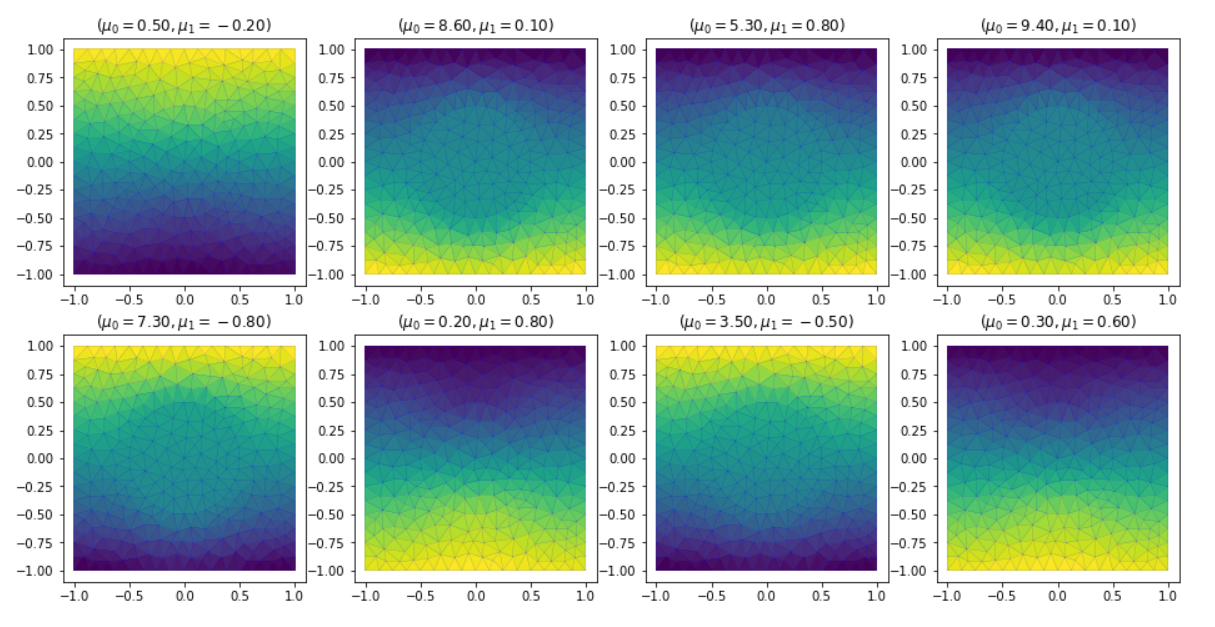
\includegraphics[width=\textwidth]{images/snapshots}
	\caption[Snapshots]{Heat distribution for the differen snapshots. }
	\label{fig:snaps}
\end{figure}

We created a reduced model from the snapshots using our algorithm.
In Figure \ref{fig:Singularvals} the value of the singular values respectively the square root of the eigenvalues is plotted.
We can see that the singular values shrink a lot between the first two modes. The following values are also shrinking but with a smaller magnitude than the first ones.

This behavior can be observed in practice. The first singular values have the biggest magnitude and decrease fast. The  modes with the singular values that fall no longer significantly can be truncated as discussed in Section \ref{sec:POD}. 

\begin{figure}[H]
	\centering
	% This file was created by matlab2tikz.
%
%The latest updates can be retrieved from
%  http://www.mathworks.com/matlabcentral/fileexchange/22022-matlab2tikz-matlab2tikz
%where you can also make suggestions and rate matlab2tikz.
%
\definecolor{mycolor1}{rgb}{0.00000,0.44700,0.74100}%
\definecolor{mycolor2}{rgb}{0.85000,0.32500,0.09800}%
\definecolor{mycolor3}{rgb}{0.92900,0.69400,0.12500}%
%
\begin{tikzpicture}

\begin{axis}[%
width=4.521in,
height=3.566in,
at={(0.758in,0.481in)},
scale only axis,
xmin=0.25,
xmax=8.25,
xlabel style={font=\color{white!15!black}},
xlabel={POD modes},
ymin=0,
ymax=950,
ylabel style={font=\color{white!15!black}},
ylabel={},
axis background/.style={fill=white},
axis x line*=bottom,
axis y line*=left,
legend style={at={(0.97,0.97)}, anchor=north east, legend cell align=left, align=left, draw=white!15!black}
]

\addplot [color=mycolor1, mark=+, mark options={solid, mycolor1, scale=2}]
table[row sep=crcr]{%
	1	874.5893 \\
	2	58.1832  \\
	3	48.2328  \\
	4	45.9105  \\
	5	35.5212  \\
	6	23.8663  \\
	7	20.6150  \\
	8	15.4926  \\
};
%\addlegendentry{Eigen values}

\end{axis}
\end{tikzpicture}%
	\caption[Singular values]{Singular values of the corresponding POD modes}
	\label{fig:Singularvals}
\end{figure}

For this simple example we didn't do the truncation.
Figure \ref{fig:reconstruct} shows a reconstucted solution with the parameter $ \bar{\mu} = (\bar{\mu}_1 , \bar{\mu}_2 )^T = ( 8 , 1 )^T $.
\begin{figure}[H]
	\centering
	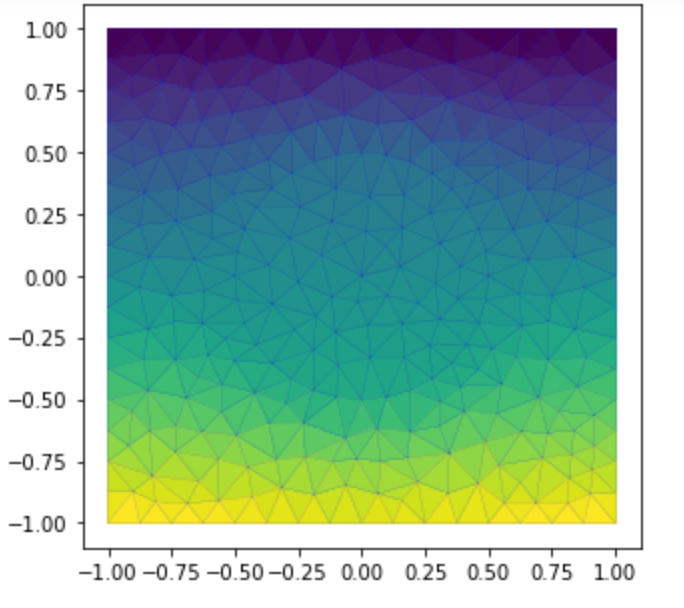
\includegraphics[width=0.38\textwidth]{images/reconstruct}
	\caption[Reduced Solution]{A solution computed with the reduced model created with \texttt{EZyRB}}
	\label{fig:reconstruct}
\end{figure}

\subsubsection{Benchmark}
With the data from tutorial 1 from \texttt{EZyRB} \cite{demo18ezyrb} we showed that the algorithm works properly, but it is not suitable to evaluate the performance.

To evaluate the performance we used a snapshot matrix with the same dimension as in Section \ref{sec:Benchmarks} and measured the time the POD class needs to compute the POD modes. This benchmark shows the performance we loose by using the python layer.

Due to issues with the cluster we had to do this benchmark on a different cluster. The new cluster has processors with 16 cores.
In Figure \ref{fig:ezybench} we can see that the measuring points increase in steps of 16 processors and not in steps of 10 like the benchmarks in Section \ref{sec:Benchmarks}.
We can still see that the implementation performed similar to the other benchmark in Figure \ref{fig:bench5} from Section \ref{sec:hybrid}.
\begin{figure}[H]
	\centering
	% This file was created by matlab2tikz.
%
%The latest updates can be retrieved from
%  http://www.mathworks.com/matlabcentral/fileexchange/22022-matlab2tikz-matlab2tikz
%where you can also make suggestions and rate matlab2tikz.
%
\definecolor{mycolor1}{rgb}{0.00000,0.44700,0.74100}%
\definecolor{mycolor2}{rgb}{0.85000,0.32500,0.09800}%
\definecolor{mycolor3}{rgb}{0.92900,0.69400,0.12500}%
%
\begin{tikzpicture}

\begin{axis}[%
width=4.521in,
height=3.566in,
at={(0.758in,0.481in)},
scale only axis,
xmin=0,
xmax=132,
xlabel style={font=\color{white!15!black}},
xlabel={Number of Processors},
ymin=0,
ymax=14.2,
ylabel style={font=\color{white!15!black}},
ylabel={Speed up},
axis background/.style={fill=white},
axis x line*=bottom,
axis y line*=left,
legend style={at={(0.03,0.97)}, anchor=north west, legend cell align=left, align=left, draw=white!15!black}
]

\addplot [color=mycolor3, mark=+, mark options={solid, mycolor3}]
table[row sep=crcr]{%
1     0.926193820542935\\
16    5.564527272810553\\
32    8.253695032798474\\
48    9.810377172379205\\
64    10.85966997160303\\
80    11.87933924922592\\
96    12.30403623120082\\
112   12.67579337348104\\
128   13.13623736917454\\
};
%\addlegendentry{EZyRB}




\end{axis}
\end{tikzpicture}%
	\caption[EZyRB Benchmark]{Benchmark integrated in the reduced order modeling framework \texttt{EZyRB}}
	\label{fig:ezybench}
\end{figure}


\newpage
\section{Conclusion}
We presented two algorithms to compute the POD in parallel.
A parallel algorithm using the singular value decomposition (SVD) and a parallel algorithm solving the eigenvalue problem of the correlation matrix (EVP).
Both algorithms performed good in case the snapshot matrix is already distributed to the different processors.
We saw that the EVP algorithm performs best, due to its limited number of operations.

For the case that the snapshot matrix is not distributed to the processors the algorithm got improved.
%We also tried to improve this algorithm for the case that the snapshot matrix is not yet distributed to the processors.
We proposed a hybrid implementation to overcome the number of communications.

Finally we  integrated the hybrid implementation into the reduced order modeling framework \texttt{EZyRB}.
We tested the new algorithm using \texttt{EZyRB} and also benchmarked the algorithm in the Python package.
With the parallel algorithm \texttt{EZyRB} can now make use af high perfomance cluster for the POD modes extraction.

In future works one could try to speed up the computation of the correlation matrix for the case that the snapshot matrix is not distributed.
Scattering the snapshot matrix to the processors is an expensive operation and slows down the overall POD computation a lot.
Instead of scattering the snapshot matrix to the processors, one could try to use Graphics Processing Units (GPU) for the computation of the correlation matrix.
GPUs are well suited these kine of operations.






